%ID: 612061
\question Consider a hash table with external chaining, using the hash function $h(x) = x \mod 10$. The table resizes when the load factor exceeds 0.75. Assume that our hash table initially has 4 buckets, and that resizing doubles the number of buckets (i.e., use the array on the right to draw the hash table after resizing). Draw out the hash table as we insert the following values:

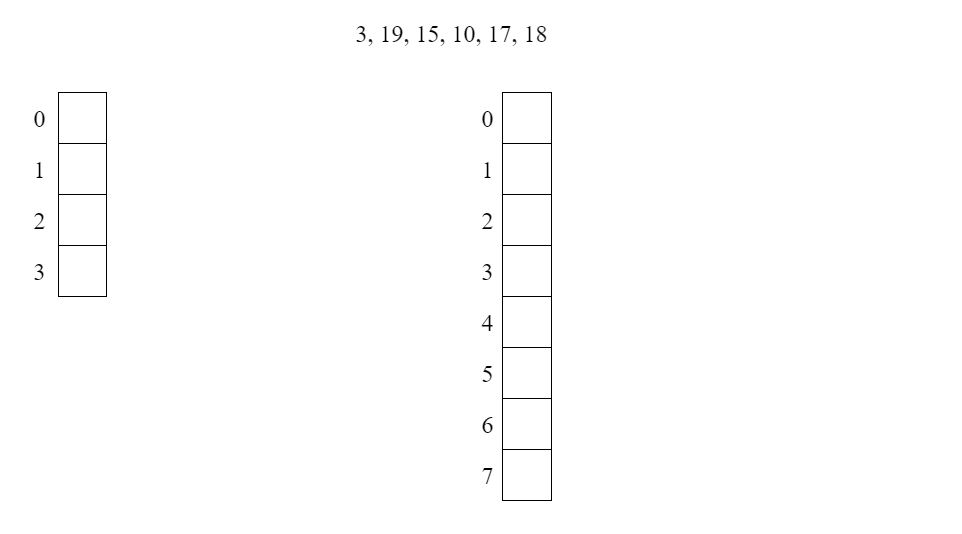
\includegraphics[scale=0.96]{topics/hashing/MockMidterm/hashing_mockmt_q1.PNG}

\begin{solution}
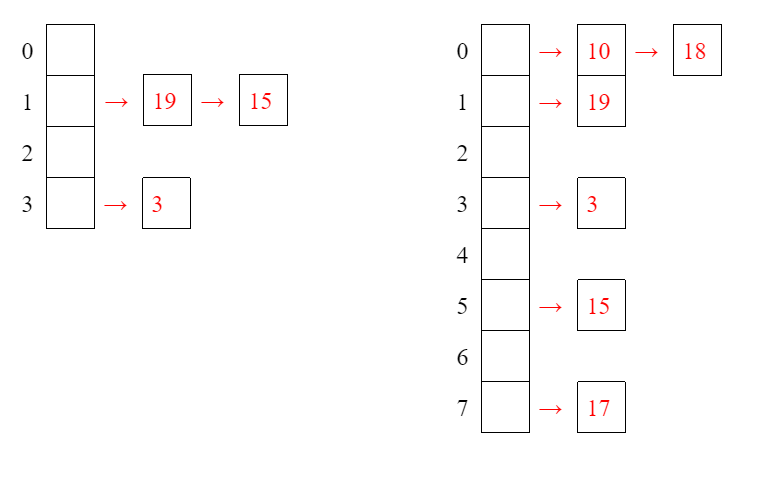
\includegraphics[scale=1]{topics/hashing/MockMidterm/hashing_mockmt_q1_sol.PNG}
\end{solution}
